\section{Unmanned aerial vehicle}
\label{sec:unmanned-aerial-vehicle}
%
%
An unmanned aerial vehicle (UAV) (commonly known as a drone) is an aircraft 
without a human pilot on board and a type of unmanned vehicle. 
UAVs are a component of an unmanned aircraft system (UAS); which include a UAV,
a ground-based controller, and a system of communications between the two.\\  
The flight of UAVs may operate with various degrees of autonomy: either under
remote control by a human operator or autonomously by on-board computers.
Compared to crewed aircraft, UAVs were originally used for missions too
dangerous for humans.\cite{budiansky2005air}\\
While they originated mostly in military applications, their use is rapidly
expanding to commercial, scientific, recreational, agricultural, policing and
surveillance, product deliveries, aerial photography, infrastructure
inspections, and drone racing.\cite{wiki:uav}
%
%
\subsection{UAV components}
\label{ssec:components}
%
Crewed and un-crewed aircraft of the same type generally have recognizably
similar physical components.  One of difference are absence the cockpit and
environmental control system or life support systems.  
Some UAVs carry payloads such as a camera or other kinds sensors smaller and 
lightweight.
Small UAVs has assumed a characteristic quad-copter design particular
recognizable, although other scheme are realizable. 
Continuous development introduced new part or revisited thus the process of
miniaturized that require less-power propulsion and increase the battery
runtime.\\
Control systems for UAVs are different for remote human control, a camera
and video link almost always replace the cockpit windows; radio-transmitted
digital commands replace physical cockpit controls. Autopilot software is used
on both crewed and uncrewed aircraft, with varying feature sets.\cite{wiki:uav}
%
%
\begin{figure}[htb]
    \centering
    \subfloat[][\emph{typical quadcopter design}.\label{subfig:quadcopter-design}]{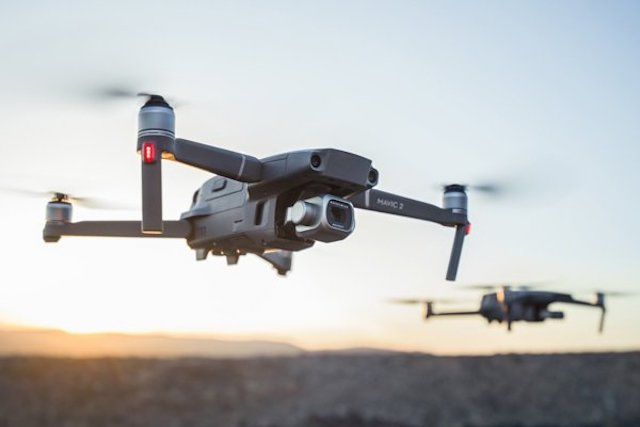
\includegraphics[width=.50\textwidth]{dji_mavic_2-1.jpg}} \\
    \subfloat[][\emph{multirotor drone design}.\label{subfig:multicopter}]{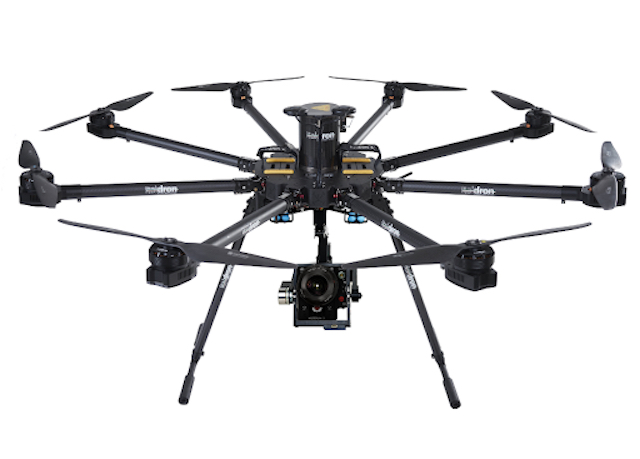
\includegraphics[width=.50\textwidth]{unnamed.jpg}} \\
    \captionsource{Example of design choices in the realization of UAVs shape}{
    \href{https://www.dji-store.it/guida-acquisto-migliori-droni-dji-per-riprese-aeree/}{DJI}; 
    \href{http://www.italdron.com/it/droni-professionali-e-accessori/droni-professionali/bigone-8hse-pro}{Italdron}}
    \label{fig:uav-design}
\end{figure}
%
%
\paragraph{Body} UAVs assume different configuration based on requirement of
task they perform for example aerial video shooting, surveys, territorial
control and many more.
Thus they are normally equipped with 4, 6, or 8 motor called quadcopter,
exacopter or octocopter.
The mainly difference that exist between different configuration is the payload
capacity that it can carry in flight.
%
\paragraph{Power supply}
Small UAVs mostly use lithium-polymer batteries (Li-Po), while larger vehicles
rely on conventional airplane engines. Scale or size of aircraft is not the
defining or limiting characteristic of energy supply for a UAV. 
Battery elimination circuitry (BEC) is used to centralize power distribution and
often harbors a microcontroller unit (MCU). Costlier switching BECs diminish
heating on the platform.\cite{wiki:uav}
%
\paragraph{Compuntig}
The hardware systems mounted on the drone have undergone an evolution in step
with the advancement of the IT sector, so much so that the analog controls have
been gradually replaced by microcontrollers up to System On Chip (SoC) with
single board cmaputer such as the Raspberry. In addition, UAVs are equipped with
flight controllers, flight controller boards and autopilots.
%
\paragraph{Sensors and Actuators}
Drone control is allowed through the cooperation of proprioceptive and
exteroceptive sensors that send their information to the central processing
unit.
The data coming from the platform measures accelerations and angular speeds
through accelerometers and gyroscopes that process and transmit the attitude
data such as orientation and position.
The GPS allows the spatial location of the aircraft on a map and to control the
route with respect to a planned trajectory. The altimeter allows you to
continuously record changes in altitude. The magnetometer is a device that
allows you to define the magnetic field vector at the point where you measure
with the drone and then obtain the orientation with respect to the North.
Knowledge and control of these measures allows the central system to allow
control of the actuators. Other more less common sensors may be present to
perform the most varied tasks.
%
\paragraph{Communications}
Most UAVs use a radio for remote control and exchange of video and other data.
The connections depending on the use cases and needs can be narrowband and
broadband. Generally, the sending and receiving of the commands is carried out
by means of a radio connection from the ground, especially for remote piloting.\\
Other connections that exploit protocols such as TCP/IP are used for sending
multimedia data such as filming areas and transmitted to mobile devices such as
smartphones, tablets and so on.
Other types of connections can be used depending on the sector of use, in fact
for the military sector these may differ to ensure greater safety and
robustness.\\ 
More and more UAVs are implementing the MAVlink protocol for the
transport of data of control and control between piloting on the ground and
aircraft.
%
%
\subsection{Autonomy}
\label{ssec:autonomy}


% ICAO classifies uncrewed aircraft as either remotely piloted aircraft or fully autonomous.[67] Actual UAVs may offer intermediate degrees of autonomy. E.g., a vehicle that is remotely piloted in most contexts may have an autonomous return-to-base operation.

% Basic autonomy comes from proprioceptive sensors. Advanced autonomy calls for situational awareness, knowledge about the environment surrounding the aircraft from exterioceptive sensors: sensor fusion integrates information from multiple sensors.[52]

% Basic principles[modifica]
% One way to achieve autonomous control employs multiple control-loop layers, as in hierarchical control systems. As of 2016 the low-layer loops (i.e. for flight control) tick as fast as 32,000 times per second, while higher-level loops may cycle once per second. The principle is to decompose the aircraft's behavior into manageable "chunks", or states, with known transitions. Hierarchical control system types range from simple scripts to finite state machines, behavior trees and hierarchical task planners. The most common control mechanism used in these layers is the PID controller which can be used to achieve hover for a quadcopter by using data from the IMU to calculate precise inputs for the electronic speed controllers and motors.[citation needed]

% Examples of mid-layer algorithms:

% Path planning: determining an optimal path for vehicle to follow while meeting mission objectives and constraints, such as obstacles or fuel requirements
% Trajectory generation (motion planning): determining control maneuvers to take in order to follow a given path or to go from one location to another[68][69]
% Trajectory regulation: constraining a vehicle within some tolerance to a trajectory
% Evolved UAV hierarchical task planners use methods like state tree searches or genetic algorithms.[70]

% Autonomy features[modifica]

% UAV's degrees of autonomy
% UAV manufacturers often build in specific autonomous operations, such as:

% Self-level: attitude stabilization on the pitch and roll axes.
% Altitude hold: The aircraft maintains its altitude using barometric or ground sensors.
% Hover/position hold: Keep level pitch and roll, stable yaw heading and altitude while maintaining position using GNSS or inertal sensors.
% Headless mode: Pitch control relative to the position of the pilot rather than relative to the vehicle's axes.
% Care-free: automatic roll and yaw control while moving horizontally
% Take-off and landing (using a variety of aircraft or ground-based sensors and systems; see also:Autoland)
% Failsafe: automatic landing or return-to-home upon loss of control signal
% Return-to-home: Fly back to the point of takeoff (often gaining altitude first to avoid possible intervening obstructions such as trees or buildings).
% Follow-me: Maintain relative position to a moving pilot or other object using GNSS, image recognition or homing beacon.
% GPS waypoint navigation: Using GNSS to navigate to an intermediate location on a travel path.
% Orbit around an object: Similar to Follow-me but continuously circle a target.
% Pre-programmed aerobatics (such as rolls and loops)